\documentclass[pdflatex,sn-mathphys-num]{sn-jnl}

\usepackage{graphicx}%
\usepackage{multirow}%
\usepackage{amsmath,amssymb,amsfonts}%
\usepackage{booktabs}%
\usepackage{xcolor}%
\usepackage{textcomp}%
\usepackage{url}%

\newcommand{\ci}[2]{[#1, #2]}   % 95\% confidence interval

\raggedbottom

\begin{document}

\title[Vietnamese Speech Translation]{Vietnamese Speech to English Text: Comparing Cascaded, Fine-Tuned and Direct Systems on FLEURS}

\author[1]{\fnm{Pham Nguyen Khanh} \sur{Nguyen} (SE200641)}
\author[1]{\fnm{Tran Thanh} \sur{Vu} (SE200433)}
\author[1]{\fnm{Ha Le Thanh} \sur{Nhan} (SE201028)}

\affil[1]{\orgdiv{Course DPL302m}, \orgname{Group 5}}

\abstract{We build and compare three systems that turn spoken Vietnamese into English text. System A is a cascade of PhoWhisper-small (speech recognition) and the pretrained OPUS-MT vi--en translation model. System B uses the same recognizer but fine-tunes OPUS-MT on ASR hypotheses paired with pseudo-translations produced by VinAI Translate v2. System C is SeamlessM4T-v2-large used zero-shot as a direct speech-to-text translation model. We take A and C as baselines and B as our proposed method. Training data is a random 55,000-sample subset of VietSpeech (61.2 h); evaluation uses the whole Vietnamese part of FLEURS (4,212 recordings, 1,978 sentences, 13.3 h), with 95\% bootstrap confidence intervals computed over unique sentences. On the main evaluation view (recordings of at most 30 s) the systems score 16.33 (A), 17.24 (B) and 27.75 (C) SacreBLEU. Fine-tuning on ASR hypotheses gives a small but real gain over A (+0.91 BLEU, CI [0.50, 1.35]) but shows no advantage over fine-tuning on clean transcripts (+0.14, CI [$-$0.14, 0.40]), and the direct system outperforms both cascades by more than 10 BLEU. Error analysis points to four main sources of loss: numbers written out as words by the recognizer, mis-transcribed proper names and loanwords, looping translations, and the domain gap between short training utterances (mean 4.0 s) and FLEURS (mean 11.3 s). A decoding-time repetition constraint (V2) removes nearly all looping outputs but improves BLEU by only 0.14. We also report model sizes, throughput on a single T4 GPU, and the limitations of the study.}

\keywords{speech translation, Vietnamese, automatic speech recognition, machine translation, FLEURS, fine-tuning}

\maketitle

%==================================================================
\section{Introduction}\label{sec:intro}

Spoken-language translation can be built in two ways. A \emph{cascade} first transcribes the audio and then translates the transcript; its parts can be trained and replaced independently, but recognition errors propagate into the translation. A \emph{direct} model maps audio to target-language text in one network and avoids that propagation, at the price of a larger model. For Vietnamese, a language with a rich tonal and diacritic system and relatively few paired speech-translation resources, it is not obvious how much a cascade can be improved by cheap adaptation, and how far it stays behind a large multilingual direct model.

This project studies that question with three systems (Section~\ref{sec:systems}): two baselines, a cascade of off-the-shelf models (A) and a direct multilingual model (C), and one proposed method (B) that adapts the translation stage of the cascade to recognizer errors. We make the following contributions.
\begin{itemize}
\item We provide a controlled comparison of A, B and C on the complete Vietnamese FLEURS set, with confidence intervals computed over unique sentences, because several recordings share the same sentence.
\item We propose training the translation model on ASR hypotheses paired with pseudo-translations, and test the idea with an ablation over the amount and the source of training data. The hypothesis that ASR-hypothesis training beats clean-transcript training is not supported by our data.
\item We analyze errors quantitatively (numbers, proper names, repetition, length, domain gap) and test one targeted fix, a repetition constraint during decoding.
\item We report resource use and state the limitations that affect how far the results can be trusted.
\end{itemize}

\section{System design}\label{sec:systems}

\begin{figure}[t]
\centering
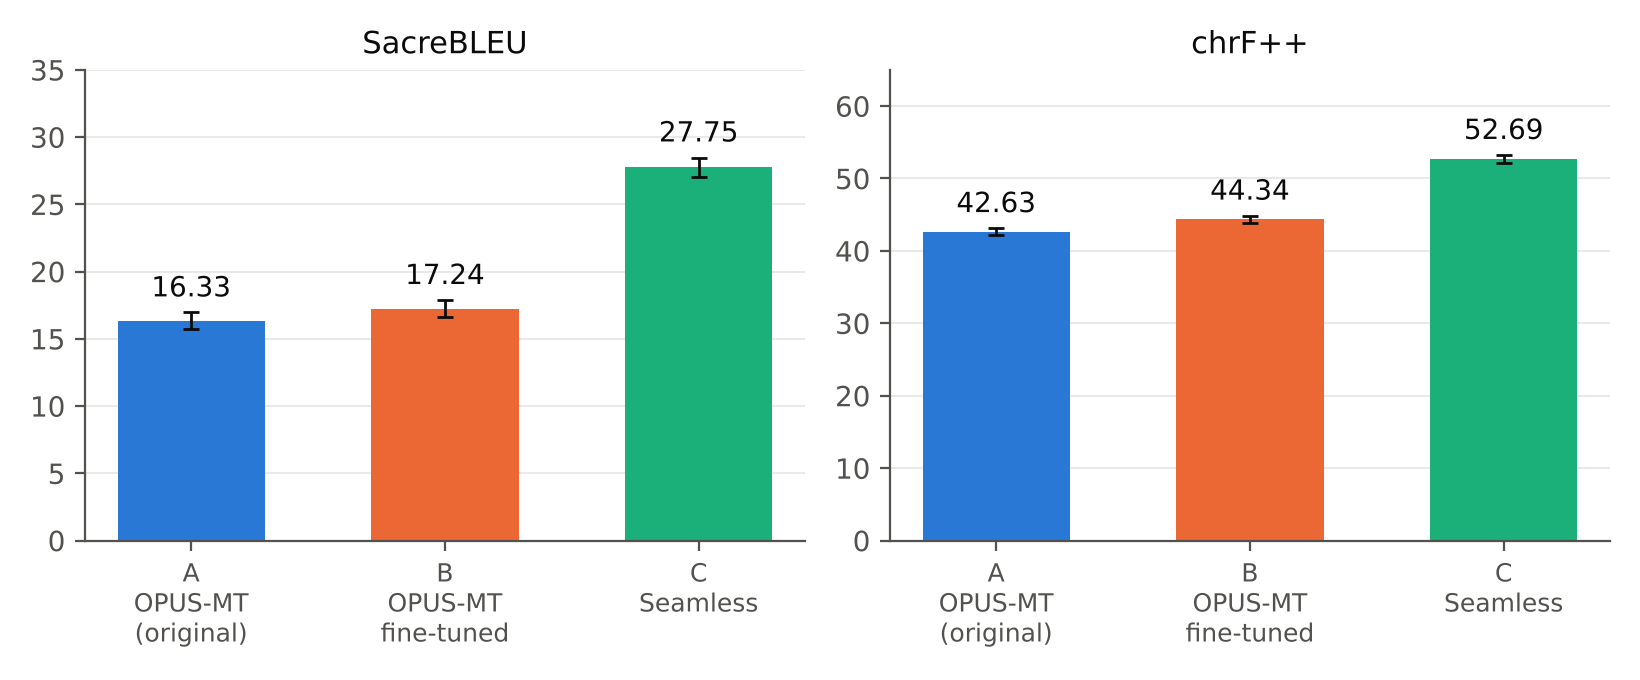
\includegraphics[width=.86\textwidth]{figs/fig_systems.png}
\caption{SacreBLEU (left) and chrF++ (right) of the three systems on FLEURS vi$\rightarrow$en (4,199 recordings of at most 30 s). Error bars are 95\% bootstrap confidence intervals over unique sentences.}\label{fig:systems}
\end{figure}

\textbf{System A (baseline 1).} PhoWhisper-small~\cite{phowhisper} transcribes the audio (beam 3), and the pretrained OPUS-MT vi--en model~\cite{opusmt} translates the transcript (beam 4). Neither model is trained further.

\textbf{System B (proposed, V1).} The same recognizer feeds an OPUS-MT model that we fine-tune on pairs (ASR hypothesis in Vietnamese, English pseudo-translation). The aim is that the translator becomes familiar with the kind of errors and the formatting (no punctuation, lower case, numbers as words) that the recognizer produces. A variant V2 changes only the decoding of the translation step (Section~\ref{sec:v2}).

\textbf{System C (baseline 2).} SeamlessM4T-v2-large~\cite{seamless} performs speech-to-text translation directly from the audio into English (beam 4), with no training on our side.

A and B share the recognizer output and differ only in the translation model; C does not use a text transcript.

\section{Data}\label{sec:data}

\subsection{Sources}

\begin{table}[t]
\caption{Data sources. No data was collected offline.}\label{tab:sources}
\begin{tabular}{@{}p{2.3cm}p{5.2cm}p{4.2cm}@{}}
\toprule
Source & Description & Size used\\
\midrule
VietSpeech (MMLab-UIT) & Online (\url{huggingface.co/datasets/NhutP/VietSpeech}); speech from several web sources, northern, central and southern accents; Apache-2.0; 16 kHz wav & 55,000 samples (61.2 h) out of 1,026,047 (over 1,100 h, 131 GB)\\
FLEURS Vietnamese & Online (Google FLEURS); read sentences with English translations (from FLORES) & 4,212 recordings, 1,978 unique sentences, 13.3 h\\
\botrule
\end{tabular}
\end{table}

\textbf{Training data.} VietSpeech provides only Vietnamese transcripts. The English side was produced by the authors by translating the Vietnamese transcripts with VinAI Translate v2 (beam 4); these are \emph{pseudo-labels}, so the quality of the fine-tuned models is bounded by the quality of these labels. We used the first 100,000 samples of the original dataset and drew 55,000 of them at random (seed 42); this size fit the GPU time budget measured on Colab (Tesla T4). The 55,000 samples were split into 5,500 for development and 49,500 for training. Nested training fractions of 25\%, 50\% and 100\% contain 12,375, 24,750 and 49,500 samples.

\textbf{Evaluation data.} We use all of FLEURS Vietnamese (train, validation and test splits) as an evaluation set, since the official test split alone has only 857 recordings (347 sentences). No system is trained on FLEURS. The metadata of both datasets leaves the sampling-rate column empty; audio is converted to mono 16 kHz.

\subsection{Cleaning and statistics}

\begin{itemize}
\item \emph{Duplicates.} VietSpeech was checked for unique identifiers; duplicate \emph{content} was not checked. In FLEURS the same sentence is read by up to three speakers (1,044 sentences have two recordings, 595 have three and 339 have one; 2.13 recordings per sentence on average), so we keep all recordings and resample by sentence when computing confidence intervals. No sentence appears in more than one FLEURS split.
\item \emph{Missing values.} Rows with empty transcripts or translations, and ASR failures, would be dropped; none occurred among the 55,000 samples. All 4,212 FLEURS rows were matched to their audio.
\item \emph{Noise and normalization.} Audio noise is not filtered. The 13 FLEURS recordings longer than 30 s (0.31\%) are truncated to 30 s and excluded from the main score. For the WER only, text is normalized (Unicode NFC, lower case, no punctuation). The pseudo-translations contain a tokenization artifact (``do n't''); we repair it with a regular expression, which changes 4,095 of 55,000 sentences (7.4\%).
\item \emph{Labelling.} No manual labelling was done, so inter-annotator agreement does not apply.
\end{itemize}

\begin{table}[t]
\caption{Data splits. FLEURS is used only for evaluation.}\label{tab:splits}
\begin{tabular}{@{}lrrr@{}}
\toprule
Set & Samples / recordings & Unique sentences & Hours\\
\midrule
VietSpeech dev & 5,500 & -- & 6.18\\
VietSpeech train & 49,500 & -- & 55.01\\
\textbf{VietSpeech total} & \textbf{55,000} & -- & \textbf{61.19}\\
\midrule
FLEURS test & 857 & 347 & 3.00\\
FLEURS validation & 361 & 149 & 1.19\\
FLEURS train & 2,994 & 1,482 & 9.08\\
\textbf{FLEURS total} & \textbf{4,212} & \textbf{1,978} & \textbf{13.27}\\
\botrule
\end{tabular}
\end{table}

\begin{table}[t]
\caption{Descriptive statistics. Every VietSpeech utterance is at most 8 s, whereas 13 FLEURS recordings exceed 30 s.}\label{tab:desc}
\begin{tabular}{@{}lrrrrrrr@{}}
\toprule
 & min & p25 & median & p75 & p95 & max & mean\\
\midrule
\multicolumn{8}{@{}l}{\emph{Duration (s)}}\\
VietSpeech (55,000) & 2.0 & 2.7 & 3.6 & 5.0 & 7.2 & 8.0 & 4.0\\
FLEURS (4,212) & 2.5 & 8.5 & 10.7 & 13.3 & 18.7 & 42.2 & 11.3\\
\midrule
\multicolumn{8}{@{}l}{\emph{Vietnamese words}}\\
VietSpeech & 3 & 10 & 13 & 18 & 27 & 44 & 14.3\\
FLEURS & 7 & 22 & 28 & 35 & 48 & 75 & 29.1\\
\botrule
\end{tabular}
\end{table}

\textbf{No class imbalance.} Recognition and translation have no class labels, so class weighting, SMOTE or focal loss do not apply. The relevant data issue is the \emph{distribution gap}: FLEURS utterances are on average 2.8 times longer (11.3 s versus 4.0 s) and have twice as many words (29.1 versus 14.3) as VietSpeech utterances, and no VietSpeech utterance is longer than 44 words whereas 5\% of FLEURS sentences have more than 48. Measures we applied are: training on ASR hypotheses instead of clean text so that training input resembles test-time input; repairing the \texttt{n't} artifact; nested training fractions to measure the effect of data size; and truncation to 30 s with a separate main view. We did \emph{not} rebalance utterance length or augment the audio.

\section{Experimental setup}\label{sec:setup}

\textbf{Environment.} All runs used an NVIDIA Tesla T4 (Google Colab) with fp16 inference, PyTorch and Hugging Face Transformers, seed 42. Beam sizes are 3 (ASR), 4 (OPUS-MT) and 4 (Seamless); inference batch sizes are 24, 64 and 8. All systems hear only the first 30 s of each recording.

\textbf{Fine-tuning (B).} The whole OPUS-MT vi--en model (72.2M parameters) is fine-tuned with \texttt{Seq2SeqTrainer}: batch size 64, learning rate $2\times10^{-5}$, weight decay 0.01, warmup of 5\% of the maximum number of steps (1,161 steps for 49,500 samples), AdamW, at most 30 epochs with early stopping on development loss (patience 5), fp16, maximum length 128 tokens. Training inputs are ASR hypotheses of VietSpeech and the repaired pseudo-translations; the development set always uses ASR hypotheses. We trained four independent runs from the original model, each with one seed: B\_100 (49,500 samples, ASR hypotheses), clean\_100 (49,500 samples, clean transcripts), B\_50 and B\_25 (ASR hypotheses, 24,750 and 12,375 samples).

\textbf{Metrics.} WER and CER for recognition; SacreBLEU (default settings, case sensitive) and chrF++ (word order 2) for translation, both on raw text. 95\% confidence intervals use 1,000 bootstrap resamples over \emph{unique sentences} (all recordings of a sentence are resampled together); differences between systems use a paired bootstrap. The \emph{main view} contains the recordings of at most 30 s (4,199 recordings, 1,974 sentences).

\section{Results}\label{sec:results}

\subsection{Comparison with published figures}\label{sec:gap}

\begin{table}[t]
\caption{Published figures and our measurements. No two rows use the same test set, so they cannot be compared directly.}\label{tab:paper}
\begin{tabular}{@{}p{2.6cm}p{3.1cm}p{3.9cm}@{}}
\toprule
Model (source) & Published & Ours (FLEURS vi)\\
\midrule
PhoWhisper-small~\cite{phowhisper} & WER 11.08 (CMV-Vi), 6.33 (VIVOS), 15.93 and 32.96 (VLSP2020 Task-1/Task-2) & WER 11.36 \ci{10.74}{11.99}; CER 7.62\\
OPUS-MT vi--en~\cite{opusmt} & BLEU 42.8, chrF 0.608 (Tatoeba-test, short sentences) & A: BLEU 16.33 \ci{15.74}{16.96}; with gold transcripts 25.91 \ci{25.08}{26.63}\\
SeamlessM4T-v2 Large~\cite{seamless} & BLEU 26.6, mean over 81 languages X$\rightarrow$eng on FLEURS S2TT (Whisper-Large-v2 + NLLB-3.3B: 22.7) & C: BLEU 27.75 \ci{27.04}{28.48}\\
\botrule
\end{tabular}
\end{table}

\emph{Recognizer.} Our WER of 11.36\% is close to the published 11.08\% but on a different test set, so it is not a reproduction. It is inflated by numerals: sentences with digits in the reference (907 sentences, 21.6\%) have WER 27.19\%, because the recognizer writes ``two thousand fifteen'' in words while the reference uses ``2015''; sentences without digits (3,292) have WER 6.81\%, close to the 6.33\% published on VIVOS (again a different set). \emph{Translator.} The published 42.8 BLEU is measured on short Tatoeba sentences; FLEURS sentences are long and written in a different register (mean 29 words). Even with gold transcripts the score is 25.91, so most of the gap is a domain gap; the recognition errors cost a further 9.6 BLEU, but this difference mixes real recognition errors with formatting differences (missing punctuation, numbers as words). \emph{Direct model.} Our 27.75 for Vietnamese is near the published mean of 26.6, which averages 81 languages; we found no Vietnamese-specific published figure. We could not verify whether FLEURS was part of Seamless's training data, which would inflate C.

\subsection{Main results}

\begin{table}[t]
\caption{Main results on 4,199 recordings of at most 30 s (1,974 sentences). On all 4,212 recordings: A 16.29, B 17.19, C 27.69. On the test split only (850 recordings): A 15.47 \ci{14.15}{16.84}; B 16.34 \ci{14.90}{17.91} ($\Delta$ +0.87 \ci{0.01}{1.88}); C 25.60 \ci{24.05}{27.26} ($\Delta$ +10.13 \ci{8.58}{11.69}).}\label{tab:main}
\begin{tabular}{@{}lcccc@{}}
\toprule
System & BLEU (95\% CI) & chrF++ & $\Delta$BLEU vs.\ A & $\Delta$chrF++\\
\midrule
A (baseline 1) & 16.33 \ci{15.74}{16.96} & 42.63 & -- & --\\
B (V1) & 17.24 \ci{16.64}{17.88} & 44.34 & +0.91 \ci{0.50}{1.35} & +1.71\\
C (baseline 2) & 27.75 \ci{27.04}{28.48} & 52.69 & +11.42 \ci{10.74}{12.14} & +10.06\\
\botrule
\end{tabular}
\end{table}

Recognition: PhoWhisper-small reaches WER 11.36\% \ci{10.74}{11.99} and CER 7.62\% (4,199 recordings); per split, test 12.16\% \ci{10.84}{13.51}, validation 10.76\% \ci{8.80}{13.06}, train 11.20\% \ci{10.40}{11.98}.

Translation: B improves on A by 0.91 BLEU (the interval excludes zero on the pooled data, but on the test split alone its lower bound is only 0.01), while C is more than 10 BLEU above both cascades. The gain of the proposed method is therefore small but real relative to A, and small relative to the distance to C.

\subsection{Training curves}

Figure~\ref{fig:loss} shows the training and development loss of the four fine-tuning runs. Training loss decreases steadily (B\_100: 1.856 to 0.767 over 11 epochs) while development loss reaches its minimum at epoch 4--6 (B\_100: 1.4645 at epoch 6) and then rises slightly (1.509 at epoch 11); the model starts to overfit after the best epoch, and early stopping selects the model at that epoch. Training loss of clean\_100 is lower from the first epoch (1.547 versus 1.856) because clean input is easier, whereas its development loss is higher because the development set always uses ASR hypotheses. Development loss is a teacher-forced loss on VietSpeech, not translation quality on FLEURS; we did not track BLEU per epoch.

\begin{figure}[t]
\centering
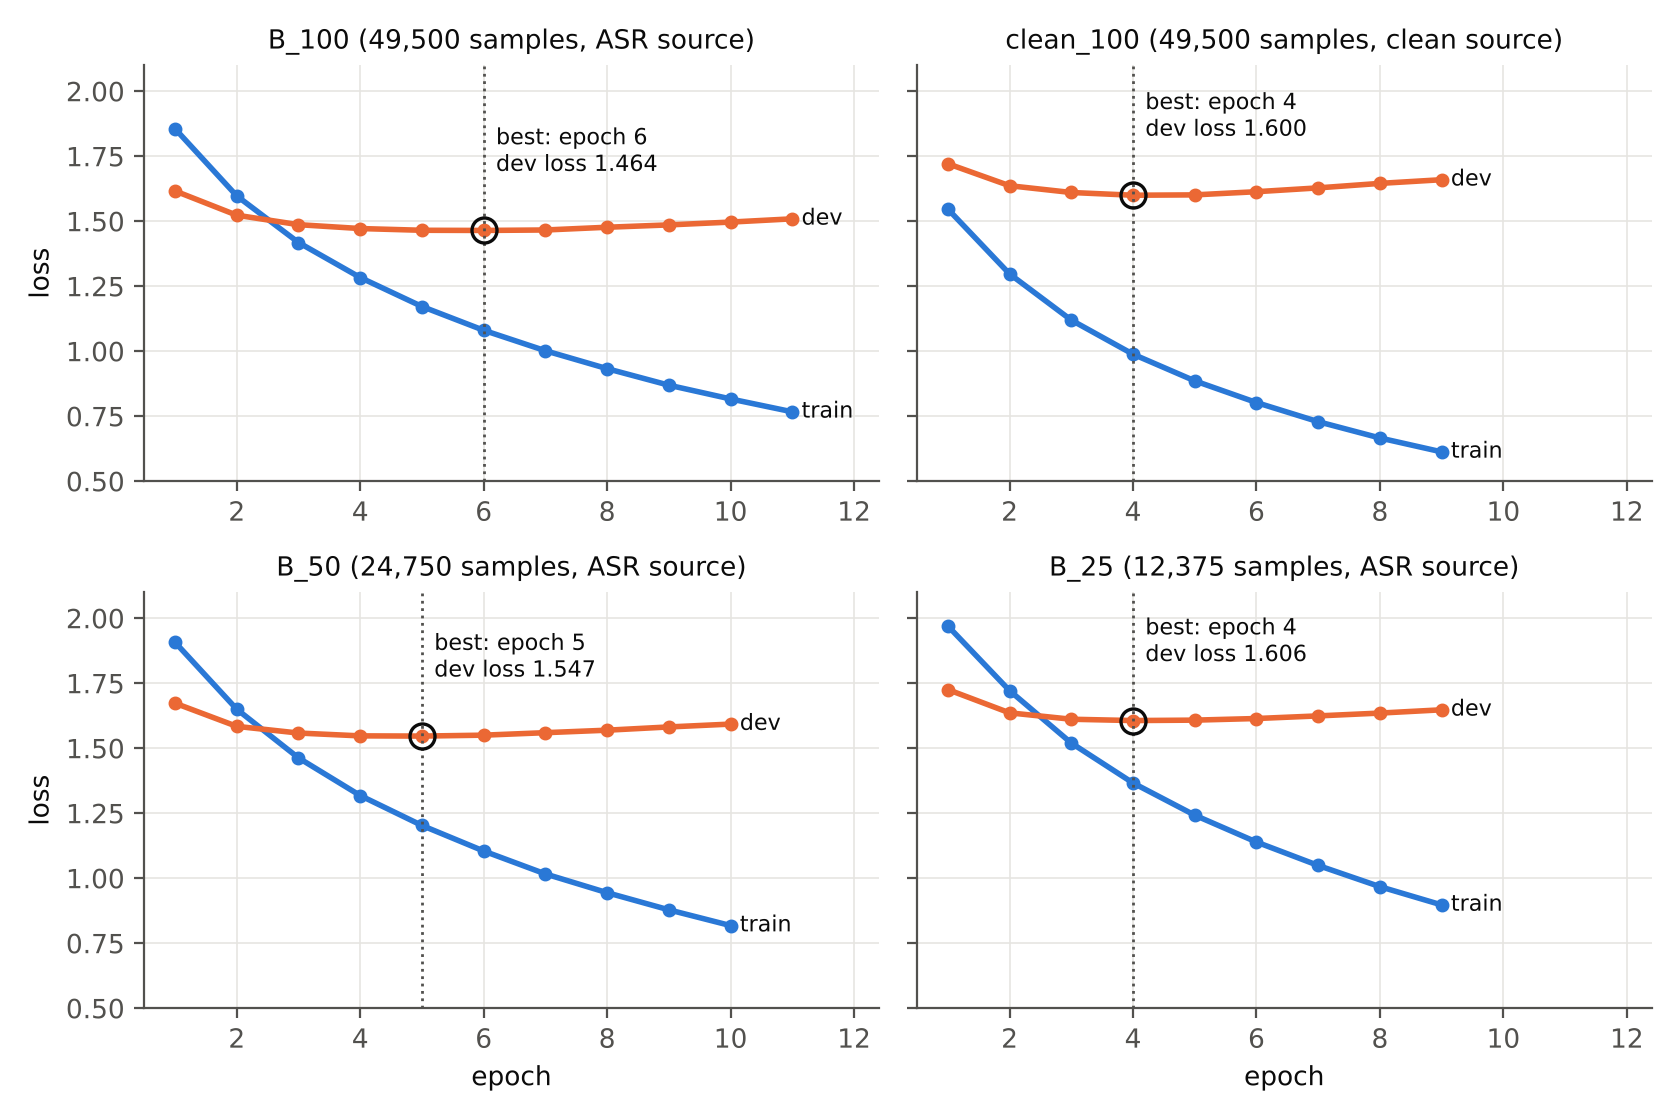
\includegraphics[width=.95\textwidth]{figs/fig_loss.png}
\caption{Training loss (blue) and development loss (orange) per epoch; circles mark the epoch with the lowest development loss. Development loss is computed on VietSpeech development data with ASR input.}\label{fig:loss}
\end{figure}

\begin{table}[t]
\caption{Training details of the four fine-tuning runs (about 62.1 minutes in total).}\label{tab:ft}
\begin{tabular}{@{}lcrccc@{}}
\toprule
Run & Input source & Train samples & Epochs run / best & Dev loss & Minutes\\
\midrule
B\_100 & ASR hypothesis & 49,500 & 11 / 6 & 1.4645 & 23.8\\
clean\_100 & clean transcript & 49,500 & 9 / 4 & 1.5999 & 19.7\\
B\_50 & ASR hypothesis & 24,750 & 10 / 5 & 1.5466 & 12.5\\
B\_25 & ASR hypothesis & 12,375 & 9 / 4 & 1.6063 & 6.2\\
\botrule
\end{tabular}
\end{table}

\subsection{Ablation: data source and data size}

\begin{table}[t]
\caption{Ablation on the main view (4,199 recordings). Each row is one independent fine-tuning run with one seed.}\label{tab:abl}
\begin{tabular}{@{}lccc@{}}
\toprule
System & BLEU (95\% CI) & chrF++ & $\Delta$BLEU vs.\ B\_100\\
\midrule
B\_25 (12,375, ASR) & 16.40 \ci{15.77}{17.01} & 43.73 & $-$0.84 \ci{$-$1.17}{$-$0.50}\\
B\_50 (24,750, ASR) & 16.86 \ci{16.24}{17.48} & 44.19 & $-$0.38 \ci{$-$0.69}{$-$0.10}\\
B\_100 (49,500, ASR) & 17.24 \ci{16.64}{17.88} & 44.34 & --\\
clean\_100 (49,500, clean) & 17.38 \ci{16.77}{18.01} & 44.62 & +0.14 \ci{$-$0.14}{0.40}\\
\botrule
\end{tabular}
\end{table}

\begin{figure}[t]
\centering
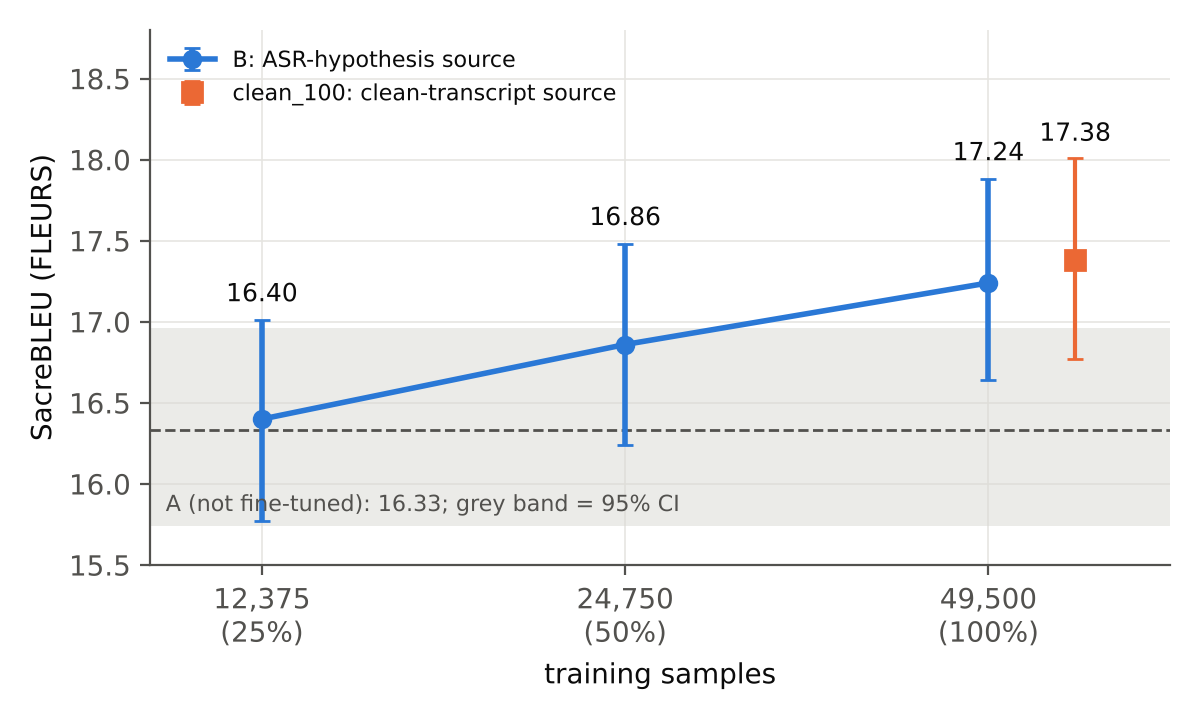
\includegraphics[width=.7\textwidth]{figs/fig_ablation.png}
\caption{BLEU against the number of training samples. The grey band is the 95\% confidence interval of A.}\label{fig:abl}
\end{figure}

More data gives a higher score (16.40, 16.86, 17.24; the differences exclude zero) and there is no sign of saturation, so more data may still help. In contrast, we found \emph{no evidence} that training on ASR hypotheses is better than training on clean transcripts (+0.14, interval containing zero); our initial hypothesis is not supported.

\section{Error analysis}\label{sec:errors}

The analysis uses the 4,199 recordings of the main view.

\textbf{Error propagation from ASR.} Grouping sentences by the WER of the recognizer, the mean chrF++ of A falls from 46.9 (WER 0, 1,220 sentences) to 31.3 (WER above 40\%, 271 sentences) and that of B from 49.0 to 32.5, whereas C is almost flat (52.8 to 51.4) because it does not pass through a text transcript (Figure~\ref{fig:wer}). Even when the transcript is perfect, A stays about 6 chrF++ points below C.

\begin{figure}[t]
\centering
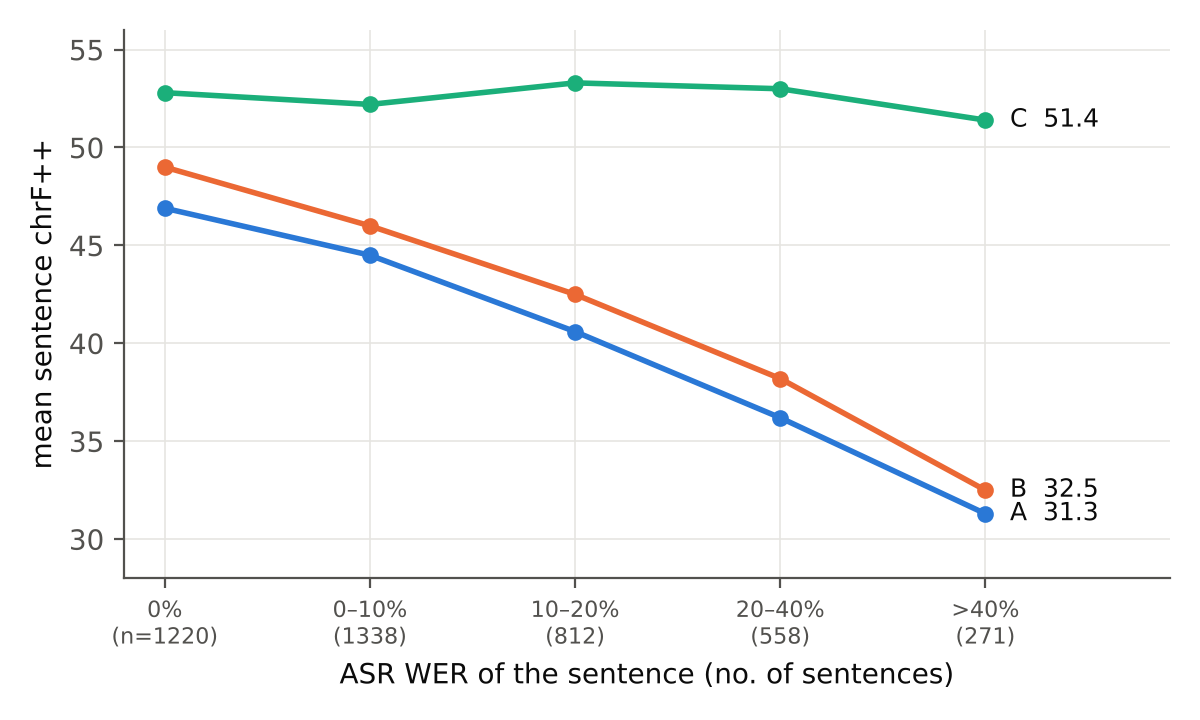
\includegraphics[width=.62\textwidth]{figs/fig_wer_bucket.png}
\caption{Mean sentence chrF++ grouped by the WER of the recognizer on that sentence.}\label{fig:wer}
\end{figure}

\textbf{Gold-input test.} Translating gold transcripts instead of ASR hypotheses raises all scores clearly (Figure~\ref{fig:gold}), but the difference confounds recognition errors with formatting differences (no punctuation, numbers as words, lower case). B\_100 with gold input (22.81) is lower than A with gold input (25.91): fine-tuning on ASR hypotheses hurts on clean input. We suspect the model has adapted to the recognizer's formatting, but we did not verify this.

\begin{figure}[t]
\centering
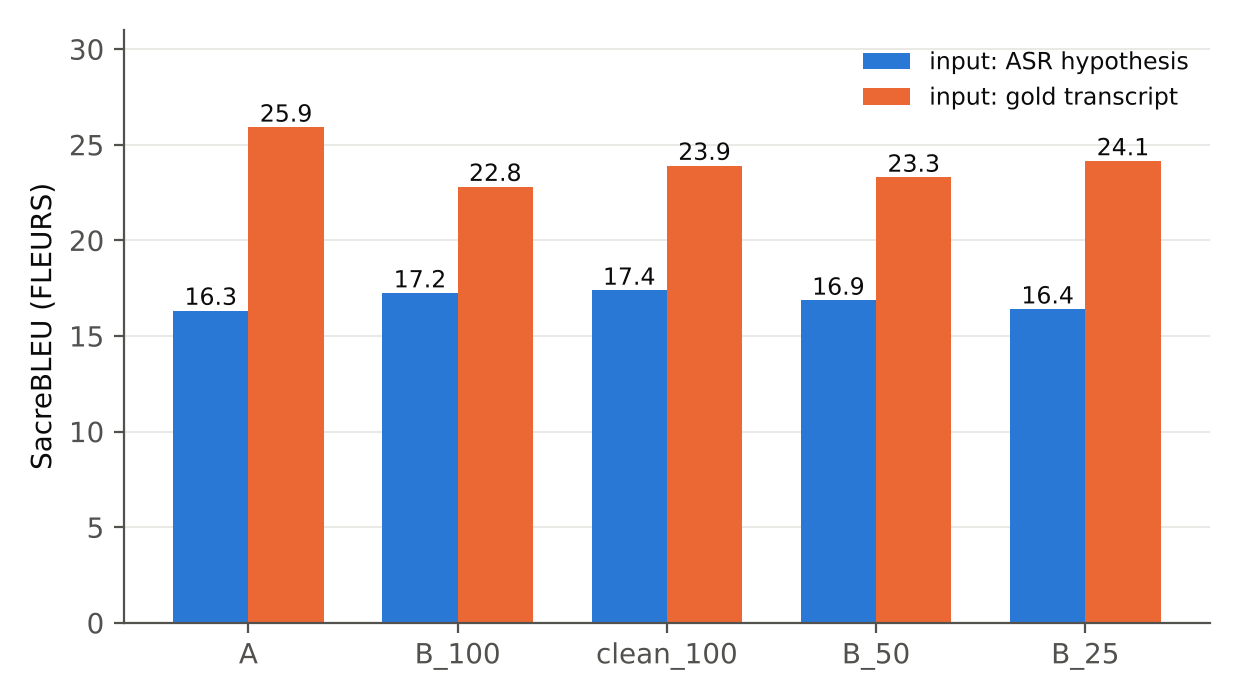
\includegraphics[width=.62\textwidth]{figs/fig_gold.png}
\caption{BLEU when the translator receives ASR hypotheses (blue) or gold transcripts (orange).}\label{fig:gold}
\end{figure}

\begin{table}[t]
\caption{Quantified error categories (4,199 recordings).}\label{tab:errors}
\begin{tabular}{@{}lccc@{}}
\toprule
Category & A & B & C\\
\midrule
BLEU, sentences with digits in the reference (907) & 11.84 & 12.06 & 29.47\\
BLEU, sentences without digits (3,292) & 17.54 & 19.06 & 27.23\\
Reference numbers present in output (of 1,378) & 115 (8\%) & 17 (1\%) & 933 (68\%)\\
Sentences with a 3-gram repeated three or more times & 16 & 31 & 11\\
Output length / reference length & 1.062 & 1.093 & 0.967\\
Outputs containing Vietnamese diacritic words & 20 & 56 & 18\\
\botrule
\end{tabular}
\end{table}

\begin{itemize}
\item \emph{Numbers (21.6\% of sentences).} The recognizer writes numbers as words, so the translation contains words (``ten thousand'') rather than digits (``10,000''). The gain of B over A is concentrated on sentences without numbers (+1.5 BLEU) and nearly zero on sentences with numbers (+0.2).
\item \emph{Proper names and loanwords.} The recognizer spells them phonetically in Vietnamese and the translator cannot repair them, whereas C hears the audio directly and usually gets them right. The share of this category was not counted (it needs manual annotation).
\item \emph{Looping translations.} B loops most often (31 sentences, against 16 for A).
\item \emph{Length and leftovers.} B produces longer output than the reference (ratio 1.093) and leaves more Vietnamese words untranslated (56 sentences against 20 for A).
\end{itemize}

\begin{table}[t]
\caption{Representative outputs (FLEURS recording identifiers in brackets). ``...'' marks omitted text.}\label{tab:examples}
\begin{tabular}{@{}p{1.6cm}p{2.5cm}p{2.0cm}p{2.0cm}p{2.0cm}@{}}
\toprule
Error & Reference & A & B & C\\
\midrule
Proper names (validation/00089) & NHK also reported that the Kashiwazaki Kariwa nuclear power plant in Niigata prefecture was operating normally. & The line of singing also informs us that the nuclear cassia plant passed through the nitrogen district & -- & The NHK also informed that the Kashiwazaki-Kariwa nuclear plant in Niigata Prefecture was operating normally.\\
\midrule
Symbols (train/01252) & Suspected cases of H5N1 in Croatia and Denmark remain unconfirmed. & No, no, no, no, ... (loop) & The suspects sing in the first year in Croatia and Denmark are still not confirmed. & The suspected H5N1 cases in Croatia and Denmark have yet to be confirmed.\\
\midrule
Loop in B (train/01539) & A contagious disease is a disease which is easily transmitted by being in the vicinity of an infected person. & The infectious disease is an easily transmitted disease in the neighborhood of the infected. & It's contagious, it's contagious, it's contagious, it's close to the sick. & An infectious disease is a disease that is easily transmitted when it is in the vicinity of an infected person.\\
\midrule
Name and number (test/00622) & Goats seem to have been first domesticated roughly 10,000 years ago in the Zagros Mountains of Iran. & ... about ten thousand years ago at the foot of Mount jaguar of iq. & ... ten thousand years ago in the mountains of Jurain in Iraq. & ... about ten thousand years ago in the Zagros Mountains of Iran.\\
\botrule
\end{tabular}
\end{table}

\section{Repetition constraint (V2)}\label{sec:v2}

\textbf{Motivation and change.} Some translations loop (16 sentences for A, 31 for B). V2 changes only one thing: \texttt{no\_repeat\_ngram\_size=3} during decoding of the translation step; the recognizer output, the models and all other settings are unchanged. Re-translating 300 sentences without the constraint reproduced V1 exactly for B (300/300) and for 296 of 300 sentences for A, so batched fp16 decoding is nearly but not perfectly repeatable.

\begin{table}[t]
\caption{V1 and V2 on the main view. On the test split alone V2 B gains +0.44 \ci{0.14}{0.81} (16.34 to 16.77).}\label{tab:v2}
\begin{tabular}{@{}lcccc@{}}
\toprule
System & BLEU (95\% CI) & chrF++ & $\Delta$BLEU vs.\ V1 & Looping sentences\\
\midrule
V1 A & 16.33 \ci{15.74}{16.96} & 42.63 & -- & 16\\
V2 A & 16.42 \ci{15.81}{17.03} & 42.67 & +0.10 \ci{0.01}{0.20} & 0\\
V1 B & 17.24 \ci{16.64}{17.88} & 44.34 & -- & 31\\
V2 B & 17.38 \ci{16.77}{17.98} & 44.40 & +0.14 \ci{0.04}{0.25} & 1\\
\botrule
\end{tabular}
\end{table}

V2 removes almost all loops but the score rises very little. A side effect is that the constraint forbids every repeated trigram, including legitimate ones, so it changed 373 outputs of B and 354 of A although only about 30 looped; one sentence with a year was translated worse. V2 was devised after reading FLEURS outputs (including the test split), so its score is subject to selection on the evaluation data, and the value 3 was not tuned.

\section{Efficiency and feasibility}\label{sec:eff}

\begin{table}[t]
\caption{Resource use on 13.26 h of audio (4,212 recordings truncated to 30 s), Tesla T4, fp16, batched inference.}\label{tab:eff}
\begin{tabular}{@{}lrrrr@{}}
\toprule
Component & Params (M) & Time (s) & VRAM (GB) & File size\\
\midrule
PhoWhisper-small (ASR) & 241.7 & 2,200 & 5.02 & 922 MB\\
OPUS-MT, original or fine-tuned & 72.2 & 56--66 & 0.96--1.15 & 274 MB\\
\textbf{A or B (ASR + translation)} & \textbf{314} & \textbf{$\approx$2,260} & \textbf{5.02} & \textbf{$\approx$1.2 GB}\\
\textbf{C: Seamless-v2 (S2TT part)} & \textbf{1,501.8} & \textbf{2,220} & \textbf{5.45} & not measured\\
\botrule
\end{tabular}
\end{table}

The real-time factor (RTF) is about 0.05 for all systems (0.046 for the recognizer after adjustment). The time of the first chunk of each stage includes model loading, so these timings are estimates after replacing that chunk by the mean of the later full chunks; the stages were not re-run. The throughput is high (about 20 times faster than real time when batched), but \emph{per-utterance latency} and single-stream performance were not measured. The Seamless part we loaded has 1.50 billion parameters, whereas the paper reports 2.3 billion for the full model~\cite{seamless}.

\textbf{Feasibility.} Technically, all three systems can be packaged as a demo on one T4-class GPU: peak VRAM is below 6 GB per system. In terms of quality, the proposed system B (and V2) improves only slightly on A and stays far from C; if translation quality matters most, C is the best choice on our data, and if a smaller model is needed, A, B or V2 are the options.

\subsection{Demo (design only)}

To make the systems usable we also prepared a demo, described here for completeness; it was \emph{not evaluated} and had not been tested end to end when this paper was written. A web interface (Gradio) accepts microphone or uploaded audio, truncates it to 30 s, and shows the Vietnamese transcript and the translations of A, B and C. A second prototype is a Chrome/Edge extension that captures the audio of a browser tab, sends 6-second chunks to a GPU server on Google Colab exposed through a temporary public tunnel, and overlays the captions on the page. Each chunk is translated independently, so sentences cut at chunk boundaries translate poorly, and the delay is at least one chunk length plus network and inference time.

\section{Limitations}\label{sec:limit}

\begin{itemize}
\item Each fine-tuning configuration was trained once (one seed); seed variance is unknown.
\item It is unknown whether FLEURS was part of the training data of SeamlessM4T-v2, which could inflate C.
\item The gold-input comparison mixes recognition errors with formatting differences.
\item WER is not normalized for numerals and is therefore inflated; BLEU and chrF++ are case sensitive and computed on raw text, which favors C (its output has capitalization and punctuation).
\item The English training labels are pseudo-translations from VinAI Translate v2; the VietSpeech subset was not checked for duplicate content.
\item V2 was designed after inspecting FLEURS outputs, including the test split, so its score carries selection effects.
\item The timings are partly estimates; per-utterance latency and behavior on spontaneous speech were not measured, and no human evaluation was done.
\item Accents (northern, central, southern) were not analyzed separately.
\end{itemize}

\section{Conclusion and future work}\label{sec:concl}

On Vietnamese FLEURS, the direct model C (27.75 BLEU) is far better than the two cascades, and adapting the translator to ASR output (B, 17.24) gives a small but real gain over the plain cascade A (16.33). The expected benefit of ASR-hypothesis fine-tuning over clean-transcript fine-tuning was not observed, and the main remaining sources of error (numerals, proper names, looping and the length gap between training and test utterances) are identified. Possible next steps, not yet tried, are: converting spelled-out numbers into digits before translation (21.6\% of sentences contain numbers, with WER 27\% versus 7\%); mixing ASR hypotheses and clean transcripts during training (B\_100 is worse than A on clean input and no better than clean\_100); concatenating short VietSpeech utterances to narrow the length gap; and repeating the experiments over several seeds.

\backmatter

\bmhead{Data and model availability}
The datasets are VietSpeech (\url{https://huggingface.co/datasets/NhutP/VietSpeech}, Apache-2.0) and FLEURS (CC-BY-4.0). The models used are \texttt{vinai/PhoWhisper-small}, \texttt{Helsinki-NLP/opus-mt-vi-en}, \texttt{facebook/seamless-m4t-v2-large} and \texttt{vinai/vinai-translate-vi2en-v2}. The fine-tuned translation model of system B can be provided by the authors on request.

\bibliography{sn-bibliography}

\end{document}
